\documentclass[twoside]{book}

% Packages required by doxygen
\usepackage{fixltx2e}
\usepackage{calc}
\usepackage{doxygen}
\usepackage[export]{adjustbox} % also loads graphicx
\usepackage{graphicx}
\usepackage[utf8]{inputenc}
\usepackage{makeidx}
\usepackage{multicol}
\usepackage{multirow}
\PassOptionsToPackage{warn}{textcomp}
\usepackage{textcomp}
\usepackage[nointegrals]{wasysym}
\usepackage[table]{xcolor}

% Font selection
\usepackage[T1]{fontenc}
\usepackage[scaled=.90]{helvet}
\usepackage{courier}
\usepackage{amssymb}
\usepackage{sectsty}
\renewcommand{\familydefault}{\sfdefault}
\allsectionsfont{%
  \fontseries{bc}\selectfont%
  \color{darkgray}%
}
\renewcommand{\DoxyLabelFont}{%
  \fontseries{bc}\selectfont%
  \color{darkgray}%
}
\newcommand{\+}{\discretionary{\mbox{\scriptsize$\hookleftarrow$}}{}{}}

% Page & text layout
\usepackage{geometry}
\geometry{%
  a4paper,%
  top=2.5cm,%
  bottom=2.5cm,%
  left=2.5cm,%
  right=2.5cm%
}
\tolerance=750
\hfuzz=15pt
\hbadness=750
\setlength{\emergencystretch}{15pt}
\setlength{\parindent}{0cm}
\setlength{\parskip}{3ex plus 2ex minus 2ex}
\makeatletter
\renewcommand{\paragraph}{%
  \@startsection{paragraph}{4}{0ex}{-1.0ex}{1.0ex}{%
    \normalfont\normalsize\bfseries\SS@parafont%
  }%
}
\renewcommand{\subparagraph}{%
  \@startsection{subparagraph}{5}{0ex}{-1.0ex}{1.0ex}{%
    \normalfont\normalsize\bfseries\SS@subparafont%
  }%
}
\makeatother

% Headers & footers
\usepackage{fancyhdr}
\pagestyle{fancyplain}
\fancyhead[LE]{\fancyplain{}{\bfseries\thepage}}
\fancyhead[CE]{\fancyplain{}{}}
\fancyhead[RE]{\fancyplain{}{\bfseries\leftmark}}
\fancyhead[LO]{\fancyplain{}{\bfseries\rightmark}}
\fancyhead[CO]{\fancyplain{}{}}
\fancyhead[RO]{\fancyplain{}{\bfseries\thepage}}
\fancyfoot[LE]{\fancyplain{}{}}
\fancyfoot[CE]{\fancyplain{}{}}
\fancyfoot[RE]{\fancyplain{}{\bfseries\scriptsize Generated by Doxygen }}
\fancyfoot[LO]{\fancyplain{}{\bfseries\scriptsize Generated by Doxygen }}
\fancyfoot[CO]{\fancyplain{}{}}
\fancyfoot[RO]{\fancyplain{}{}}
\renewcommand{\footrulewidth}{0.4pt}
\renewcommand{\chaptermark}[1]{%
  \markboth{#1}{}%
}
\renewcommand{\sectionmark}[1]{%
  \markright{\thesection\ #1}%
}

% Indices & bibliography
\usepackage{natbib}
\usepackage[titles]{tocloft}
\setcounter{tocdepth}{3}
\setcounter{secnumdepth}{5}
\makeindex

% Hyperlinks (required, but should be loaded last)
\usepackage{ifpdf}
\ifpdf
  \usepackage[pdftex,pagebackref=true]{hyperref}
\else
  \usepackage[ps2pdf,pagebackref=true]{hyperref}
\fi
\hypersetup{%
  colorlinks=true,%
  linkcolor=blue,%
  citecolor=blue,%
  unicode%
}

% Custom commands
\newcommand{\clearemptydoublepage}{%
  \newpage{\pagestyle{empty}\cleardoublepage}%
}

\usepackage{caption}
\captionsetup{labelsep=space,justification=centering,font={bf},singlelinecheck=off,skip=4pt,position=top}

%===== C O N T E N T S =====

\begin{document}

% Titlepage & ToC
\hypersetup{pageanchor=false,
             bookmarksnumbered=true,
             pdfencoding=unicode
            }
\pagenumbering{alph}
\begin{titlepage}
\vspace*{7cm}
\begin{center}%
{\Large Gnome Text\+Box }\\
\vspace*{1cm}
{\large Generated by Doxygen 1.8.13}\\
\end{center}
\end{titlepage}
\clearemptydoublepage
\pagenumbering{roman}
\tableofcontents
\clearemptydoublepage
\pagenumbering{arabic}
\hypersetup{pageanchor=true}

%--- Begin generated contents ---
\chapter{Overview}
\label{index}\hypertarget{index}{}Text\+Box is a graphical application that provides all the functionality of a modern pseudo-\/terminal without the burden of emulating a terminal. Text\+Box also provides new functionality such as, event driven key binding, H\+T\+ML like markup, embedded images, separate read and write positions, dynamic line oriented coordinates, and line editing semantics. Note you will need \href{https://codrod.github.io/libtb/index.html}{\tt libtb} to use a Text\+Box in your application. This implementation of Text\+Box uses the gtkmm bindings for the G\+I\+MP Toolkit (G\+TK). 
\chapter{Gnome Text\+Box}
\label{a00057}
\Hypertarget{a00057}
\subsubsection*{Overview}

Text\+Box is a graphical application that provides all the functionality of a modern pseudo-\/terminal without the burden of emulating a terminal. Text\+Box also provides new functionality such as, event driven key binding, H\+T\+ML like markup, embedded images, separate read and write positions, dynamic line oriented coordinates, and line editing semantics. Note you will need \href{https://codrod.github.io/libtb/index.html}{\tt libtb} to use a Text\+Box in your application. This implementation of Text\+Box uses the gtkmm bindings for the G\+I\+MP Toolkit (G\+TK).

\subsubsection*{Documentation}

Documentation is generated by Doxygen and hosted on \href{https://codrod.github.io/gtb/index.html}{\tt Git\+Hub Pages}.

\subsubsection*{Build Instructions}


\begin{DoxyItemize}
\item make
\item make docs
\end{DoxyItemize}

\subsubsection*{Development Status}


\begin{DoxyItemize}
\item cursor control/positioning -\/ completed
\item insert output -\/ completed
\item clear output -\/ completed
\item scroll output -\/ completed
\item edit line -\/ completed
\item text markup -\/ in progress
\item embedded images -\/ in progress
\item event driven key binding -\/ not started
\end{DoxyItemize}

\subsubsection*{Development Plan}


\begin{DoxyEnumerate}
\item Add unit testing
\item Add backwards compatible termcap and ncurses support
\item Improve documentation
\item Complete current features
\item Windows port 
\end{DoxyEnumerate}
\chapter{Hierarchical Index}
\section{Class Hierarchy}
This inheritance list is sorted roughly, but not completely, alphabetically\+:\begin{DoxyCompactList}
\item Application\+Window\begin{DoxyCompactList}
\item \contentsline{section}{G\+TB\+:\+:Window}{\pageref{a00036}}{}
\end{DoxyCompactList}
\item \contentsline{section}{G\+TB\+:\+:Controller}{\pageref{a00048}}{}
\item \contentsline{section}{G\+TB\+:\+:coord}{\pageref{a00024}}{}
\item exception\begin{DoxyCompactList}
\item \contentsline{section}{G\+TB\+:\+:Error}{\pageref{a00012}}{}
\item \contentsline{section}{G\+TB\+:\+:Fatal\+Error}{\pageref{a00016}}{}
\end{DoxyCompactList}
\item \contentsline{section}{G\+TB\+:\+:Inputer}{\pageref{a00044}}{}
\item \contentsline{section}{G\+TB\+:\+:Outputer}{\pageref{a00040}}{}
\item \contentsline{section}{G\+TB\+:\+:Sequence}{\pageref{a00020}}{}
\item \contentsline{section}{G\+TB\+:\+:Tag}{\pageref{a00028}}{}
\item \contentsline{section}{G\+TB\+:\+:Tag\+Area}{\pageref{a00032}}{}
\end{DoxyCompactList}

\chapter{Class Index}
\section{Class List}
Here are the classes, structs, unions and interfaces with brief descriptions\+:\begin{DoxyCompactList}
\item\contentsline{section}{\hyperlink{a00048}{G\+T\+B\+::\+Controller} }{\pageref{a00048}}{}
\item\contentsline{section}{\hyperlink{a00024}{G\+T\+B\+::coord} }{\pageref{a00024}}{}
\item\contentsline{section}{\hyperlink{a00012}{G\+T\+B\+::\+Error} }{\pageref{a00012}}{}
\item\contentsline{section}{\hyperlink{a00016}{G\+T\+B\+::\+Fatal\+Error} }{\pageref{a00016}}{}
\item\contentsline{section}{\hyperlink{a00044}{G\+T\+B\+::\+Inputer} }{\pageref{a00044}}{}
\item\contentsline{section}{\hyperlink{a00040}{G\+T\+B\+::\+Outputer} }{\pageref{a00040}}{}
\item\contentsline{section}{\hyperlink{a00020}{G\+T\+B\+::\+Sequence} }{\pageref{a00020}}{}
\item\contentsline{section}{\hyperlink{a00028}{G\+T\+B\+::\+Tag} }{\pageref{a00028}}{}
\item\contentsline{section}{\hyperlink{a00032}{G\+T\+B\+::\+Tag\+Area} }{\pageref{a00032}}{}
\item\contentsline{section}{\hyperlink{a00036}{G\+T\+B\+::\+Window} }{\pageref{a00036}}{}
\end{DoxyCompactList}

\chapter{File Index}
\section{File List}
Here is a list of all documented files with brief descriptions\+:\begin{DoxyCompactList}
\item\contentsline{section}{\hyperlink{a00005}{gtb.\+h} \\*Header file for Gnome Text\+Box }{\pageref{a00005}}{}
\end{DoxyCompactList}

\chapter{Class Documentation}
\hypertarget{a00048}{}\section{G\+TB\+:\+:Controller Class Reference}
\label{a00048}\index{G\+T\+B\+::\+Controller@{G\+T\+B\+::\+Controller}}


Collaboration diagram for G\+TB\+:\+:Controller\+:\nopagebreak
\begin{figure}[H]
\begin{center}
\leavevmode
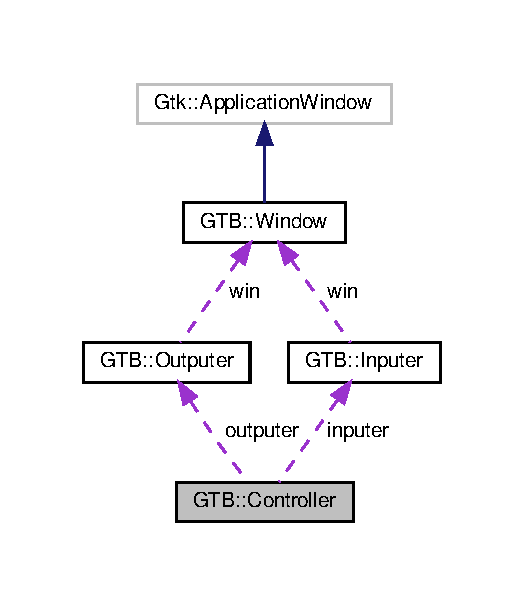
\includegraphics[width=252pt]{a00046}
\end{center}
\end{figure}
\subsection*{Public Member Functions}
\begin{DoxyCompactItemize}
\item 
\mbox{\Hypertarget{a00048_a6e66408f89303e9684a4ba88e21212e2}\label{a00048_a6e66408f89303e9684a4ba88e21212e2}} 
{\bfseries Controller} (\hyperlink{a00044}{Inputer} \&inputer, \hyperlink{a00040}{Outputer} \&outputer)
\item 
\mbox{\Hypertarget{a00048_a21117179f6c38e98c5f7f27f92353f56}\label{a00048_a21117179f6c38e98c5f7f27f92353f56}} 
bool {\bfseries controller} (const Glib\+::\+I\+O\+Condition cond)
\item 
\mbox{\Hypertarget{a00048_a917a873c1238b3e84c40492fa2fb8458}\label{a00048_a917a873c1238b3e84c40492fa2fb8458}} 
Glib\+::\+I\+O\+Status {\bfseries get} (Glib\+::ustring \&seq)
\item 
\mbox{\Hypertarget{a00048_a87d9bc4196a63f521a1a26370dc9d599}\label{a00048_a87d9bc4196a63f521a1a26370dc9d599}} 
int {\bfseries put} (Glib\+::ustring seq)
\item 
\mbox{\Hypertarget{a00048_a4c711a4acf28d83caa66de761ef7ce08}\label{a00048_a4c711a4acf28d83caa66de761ef7ce08}} 
bool {\bfseries scroll} ()
\item 
\mbox{\Hypertarget{a00048_ad8b9cbaa251de2d2d6fe57dd02318df8}\label{a00048_ad8b9cbaa251de2d2d6fe57dd02318df8}} 
Glib\+::ustring {\bfseries exec} (\hyperlink{a00020}{Sequence} seq)
\item 
\mbox{\Hypertarget{a00048_a947de364ba1bf3d80382241af2655d69}\label{a00048_a947de364ba1bf3d80382241af2655d69}} 
Glib\+::ustring {\bfseries dcs\+\_\+setup} (\hyperlink{a00020}{Sequence} seq)
\item 
\mbox{\Hypertarget{a00048_ae464f9974723e995a255ffa06ad0c956}\label{a00048_ae464f9974723e995a255ffa06ad0c956}} 
Glib\+::ustring {\bfseries dcs\+\_\+move} (\hyperlink{a00020}{Sequence} seq)
\item 
\mbox{\Hypertarget{a00048_a3d41ede153f82fcdfd97e2065e0e2c8a}\label{a00048_a3d41ede153f82fcdfd97e2065e0e2c8a}} 
Glib\+::ustring {\bfseries dcs\+\_\+find} (\hyperlink{a00020}{Sequence} seq)
\item 
\mbox{\Hypertarget{a00048_ad06e95f8672f3b529826ab4bf36fe0f7}\label{a00048_ad06e95f8672f3b529826ab4bf36fe0f7}} 
Glib\+::ustring {\bfseries dcs\+\_\+scroll} (\hyperlink{a00020}{Sequence} seq)
\item 
\mbox{\Hypertarget{a00048_ad82a254681cc287a260fd0eeea225804}\label{a00048_ad82a254681cc287a260fd0eeea225804}} 
Glib\+::ustring {\bfseries dcs\+\_\+insert} (\hyperlink{a00020}{Sequence} seq)
\item 
\mbox{\Hypertarget{a00048_a138d596d5c6419ce8e7b8fe0a3892dc4}\label{a00048_a138d596d5c6419ce8e7b8fe0a3892dc4}} 
Glib\+::ustring {\bfseries dcs\+\_\+edit} (\hyperlink{a00020}{Sequence} seq)
\item 
\mbox{\Hypertarget{a00048_a492baf19b2f0af59cfaa2e6c1d7e0de7}\label{a00048_a492baf19b2f0af59cfaa2e6c1d7e0de7}} 
Glib\+::ustring {\bfseries dcs\+\_\+clear} (\hyperlink{a00020}{Sequence} seq)
\item 
\mbox{\Hypertarget{a00048_a7b77ee0ab4692cf5b787df9018359ecf}\label{a00048_a7b77ee0ab4692cf5b787df9018359ecf}} 
Glib\+::ustring {\bfseries dcs\+\_\+embed} (\hyperlink{a00020}{Sequence} seq)
\end{DoxyCompactItemize}
\subsection*{Public Attributes}
\begin{DoxyCompactItemize}
\item 
\mbox{\Hypertarget{a00048_a4fc2df37ff31426309ab5b126ed08fe5}\label{a00048_a4fc2df37ff31426309ab5b126ed08fe5}} 
\hyperlink{a00040}{Outputer} \& {\bfseries outputer}
\item 
\mbox{\Hypertarget{a00048_a5da43092c0b6387513d66846127822ac}\label{a00048_a5da43092c0b6387513d66846127822ac}} 
\hyperlink{a00044}{Inputer} \& {\bfseries inputer}
\item 
\mbox{\Hypertarget{a00048_ae6f910dbf841326fae3b4b203be52eda}\label{a00048_ae6f910dbf841326fae3b4b203be52eda}} 
Glib\+::\+Ref\+Ptr$<$ Glib\+::\+I\+O\+Channel $>$ {\bfseries io\+\_\+channel}
\item 
\mbox{\Hypertarget{a00048_acaafbd26faf38b2e2313e4aeabdef4d1}\label{a00048_acaafbd26faf38b2e2313e4aeabdef4d1}} 
int {\bfseries in}
\item 
\mbox{\Hypertarget{a00048_a782ca1e6f668e7c26664e5bf393407cd}\label{a00048_a782ca1e6f668e7c26664e5bf393407cd}} 
int {\bfseries out}
\item 
\mbox{\Hypertarget{a00048_a366878f4a7789d22fe82c89b940b38dc}\label{a00048_a366878f4a7789d22fe82c89b940b38dc}} 
Gtk\+::\+Text\+Iter {\bfseries scroll\+\_\+pos}
\item 
\mbox{\Hypertarget{a00048_a45bc17b8a501934841af9d288a75021c}\label{a00048_a45bc17b8a501934841af9d288a75021c}} 
sem\+\_\+t $\ast$ {\bfseries lock}
\end{DoxyCompactItemize}


The documentation for this class was generated from the following file\+:\begin{DoxyCompactItemize}
\item 
\hyperlink{a00005}{gtb.\+h}\end{DoxyCompactItemize}

\hypertarget{a00024}{}\section{G\+TB\+:\+:coord Class Reference}
\label{a00024}\index{G\+T\+B\+::coord@{G\+T\+B\+::coord}}
\subsection*{Public Member Functions}
\begin{DoxyCompactItemize}
\item 
\mbox{\Hypertarget{a00024_a06ca8c21b8c157e8ef387dd63879769e}\label{a00024_a06ca8c21b8c157e8ef387dd63879769e}} 
{\bfseries coord} (long long int x, long long int y)
\end{DoxyCompactItemize}
\subsection*{Public Attributes}
\begin{DoxyCompactItemize}
\item 
\mbox{\Hypertarget{a00024_a35f83d59002019943f5166bf81445d42}\label{a00024_a35f83d59002019943f5166bf81445d42}} 
long long int {\bfseries x}
\item 
\mbox{\Hypertarget{a00024_ac17a3b1e5c13fc9eaad723c95cb1059b}\label{a00024_ac17a3b1e5c13fc9eaad723c95cb1059b}} 
long long int {\bfseries y}
\end{DoxyCompactItemize}


The documentation for this class was generated from the following file\+:\begin{DoxyCompactItemize}
\item 
\hyperlink{a00005}{gtb.\+h}\end{DoxyCompactItemize}

\hypertarget{a00012}{}\section{G\+TB\+:\+:Error Class Reference}
\label{a00012}\index{G\+T\+B\+::\+Error@{G\+T\+B\+::\+Error}}


Inheritance diagram for G\+TB\+:\+:Error\+:\nopagebreak
\begin{figure}[H]
\begin{center}
\leavevmode
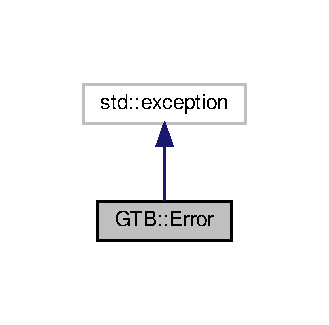
\includegraphics[width=158pt]{a00011}
\end{center}
\end{figure}


Collaboration diagram for G\+TB\+:\+:Error\+:\nopagebreak
\begin{figure}[H]
\begin{center}
\leavevmode
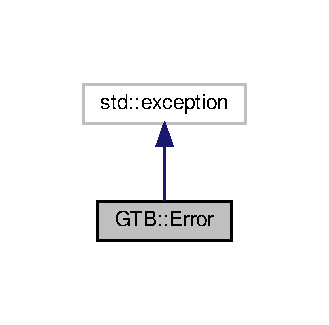
\includegraphics[width=158pt]{a00010}
\end{center}
\end{figure}
\subsection*{Public Member Functions}
\begin{DoxyCompactItemize}
\item 
\mbox{\Hypertarget{a00012_a031a14b03c0216488ba8bcca38a3ac8d}\label{a00012_a031a14b03c0216488ba8bcca38a3ac8d}} 
{\bfseries Error} (const std\+::string \&str)
\item 
\mbox{\Hypertarget{a00012_a2a8e6b4c9abf65b57741cb14b0eb2c39}\label{a00012_a2a8e6b4c9abf65b57741cb14b0eb2c39}} 
{\bfseries Error} (const char $\ast$str)
\item 
\mbox{\Hypertarget{a00012_ab9fee344d3f1be089c12e50e8f49297d}\label{a00012_ab9fee344d3f1be089c12e50e8f49297d}} 
virtual const char $\ast$ {\bfseries what} () const noexcept
\end{DoxyCompactItemize}
\subsection*{Public Attributes}
\begin{DoxyCompactItemize}
\item 
\mbox{\Hypertarget{a00012_a6b8ba43c75374c925d6c439cef67cedf}\label{a00012_a6b8ba43c75374c925d6c439cef67cedf}} 
std\+::string {\bfseries msg}
\end{DoxyCompactItemize}


The documentation for this class was generated from the following file\+:\begin{DoxyCompactItemize}
\item 
\hyperlink{a00005}{gtb.\+h}\end{DoxyCompactItemize}

\hypertarget{a00016}{}\section{G\+TB\+:\+:Fatal\+Error Class Reference}
\label{a00016}\index{G\+T\+B\+::\+Fatal\+Error@{G\+T\+B\+::\+Fatal\+Error}}


Inheritance diagram for G\+TB\+:\+:Fatal\+Error\+:\nopagebreak
\begin{figure}[H]
\begin{center}
\leavevmode
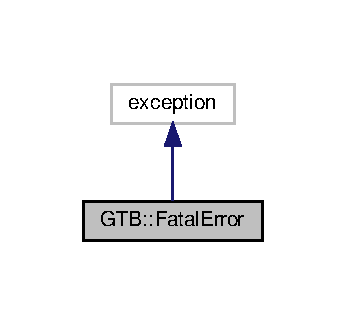
\includegraphics[width=166pt]{a00015}
\end{center}
\end{figure}


Collaboration diagram for G\+TB\+:\+:Fatal\+Error\+:\nopagebreak
\begin{figure}[H]
\begin{center}
\leavevmode
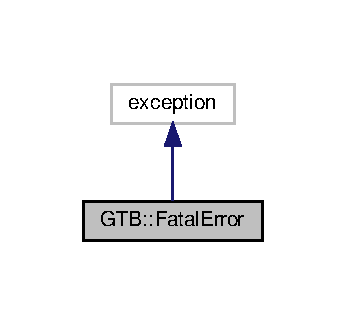
\includegraphics[width=166pt]{a00014}
\end{center}
\end{figure}
\subsection*{Public Member Functions}
\begin{DoxyCompactItemize}
\item 
\mbox{\Hypertarget{a00016_add7315c779227e83ff575705aaa8199e}\label{a00016_add7315c779227e83ff575705aaa8199e}} 
{\bfseries Fatal\+Error} (const std\+::string \&str)
\item 
\mbox{\Hypertarget{a00016_a217f06adacb94fc8015d1b356110f04a}\label{a00016_a217f06adacb94fc8015d1b356110f04a}} 
{\bfseries Fatal\+Error} (const char $\ast$str)
\item 
\mbox{\Hypertarget{a00016_aa3c9e54856b7fa4787499e796cef745c}\label{a00016_aa3c9e54856b7fa4787499e796cef745c}} 
virtual const char $\ast$ {\bfseries what} () const noexcept
\end{DoxyCompactItemize}
\subsection*{Public Attributes}
\begin{DoxyCompactItemize}
\item 
\mbox{\Hypertarget{a00016_af383e83dac310b9bf87b759d08171d5f}\label{a00016_af383e83dac310b9bf87b759d08171d5f}} 
std\+::string {\bfseries msg}
\end{DoxyCompactItemize}


The documentation for this class was generated from the following file\+:\begin{DoxyCompactItemize}
\item 
\hyperlink{a00005}{gtb.\+h}\end{DoxyCompactItemize}

\hypertarget{a00044}{}\section{G\+TB\+:\+:Inputer Class Reference}
\label{a00044}\index{G\+T\+B\+::\+Inputer@{G\+T\+B\+::\+Inputer}}


Collaboration diagram for G\+TB\+:\+:Inputer\+:\nopagebreak
\begin{figure}[H]
\begin{center}
\leavevmode
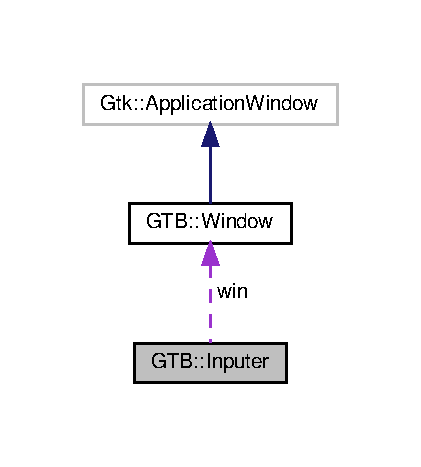
\includegraphics[width=202pt]{a00042}
\end{center}
\end{figure}
\subsection*{Public Member Functions}
\begin{DoxyCompactItemize}
\item 
\mbox{\Hypertarget{a00044_ae2a8db83378f9ba8bf19e4bf8531cf7d}\label{a00044_ae2a8db83378f9ba8bf19e4bf8531cf7d}} 
{\bfseries Inputer} (\hyperlink{a00036}{Window} \&win)
\item 
\mbox{\Hypertarget{a00044_a2cb5c87ba92fe20f19996490a8096680}\label{a00044_a2cb5c87ba92fe20f19996490a8096680}} 
bool {\bfseries inputer} (Gdk\+Event\+Key $\ast$event)
\item 
\mbox{\Hypertarget{a00044_a4da7991373f7f076f20ad31074c4fb8f}\label{a00044_a4da7991373f7f076f20ad31074c4fb8f}} 
\hyperlink{a00044}{Inputer} \& {\bfseries move} (\hyperlink{a00024}{coord} pos)
\item 
\mbox{\Hypertarget{a00044_a5e7f591d5e30de5897274e5d16f13094}\label{a00044_a5e7f591d5e30de5897274e5d16f13094}} 
\hyperlink{a00024}{coord} {\bfseries find} ()
\item 
\mbox{\Hypertarget{a00044_a20d77d58027c7424b66eef37f37d38fc}\label{a00044_a20d77d58027c7424b66eef37f37d38fc}} 
\hyperlink{a00044}{Inputer} \& {\bfseries edit} (Glib\+::ustring str)
\end{DoxyCompactItemize}
\subsection*{Public Attributes}
\begin{DoxyCompactItemize}
\item 
\mbox{\Hypertarget{a00044_ac4b9dc02472ac3dfbc1f782ad199f544}\label{a00044_ac4b9dc02472ac3dfbc1f782ad199f544}} 
\hyperlink{a00036}{Window} \& {\bfseries win}
\item 
\mbox{\Hypertarget{a00044_aa932c88c46ea54581eecef2e549e0d12}\label{a00044_aa932c88c46ea54581eecef2e549e0d12}} 
int {\bfseries in} \mbox{[}2\mbox{]}
\end{DoxyCompactItemize}


The documentation for this class was generated from the following file\+:\begin{DoxyCompactItemize}
\item 
\hyperlink{a00005}{gtb.\+h}\end{DoxyCompactItemize}

\hypertarget{a00040}{}\section{G\+TB\+:\+:Outputer Class Reference}
\label{a00040}\index{G\+T\+B\+::\+Outputer@{G\+T\+B\+::\+Outputer}}


Collaboration diagram for G\+TB\+:\+:Outputer\+:\nopagebreak
\begin{figure}[H]
\begin{center}
\leavevmode
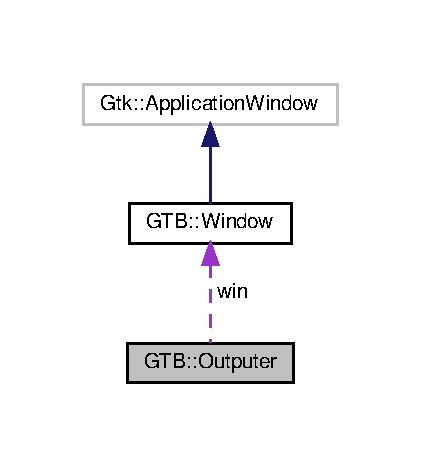
\includegraphics[width=202pt]{a00038}
\end{center}
\end{figure}
\subsection*{Public Member Functions}
\begin{DoxyCompactItemize}
\item 
\mbox{\Hypertarget{a00040_a1ed68f578cf79072628c058a77ac526f}\label{a00040_a1ed68f578cf79072628c058a77ac526f}} 
{\bfseries Outputer} (\hyperlink{a00036}{Window} \&win)
\item 
\mbox{\Hypertarget{a00040_ab409d72eb7c8d60261e8b451eb3a9031}\label{a00040_ab409d72eb7c8d60261e8b451eb3a9031}} 
bool {\bfseries outputer} (const Glib\+::\+I\+O\+Condition cond)
\item 
\mbox{\Hypertarget{a00040_afcce9d49fc8a6e85e58bc9c10ba78837}\label{a00040_afcce9d49fc8a6e85e58bc9c10ba78837}} 
Glib\+::\+I\+O\+Status {\bfseries get\+\_\+line} (Glib\+::ustring \&text)
\item 
\mbox{\Hypertarget{a00040_ab36a8f86bc8f2dd5d0cebb298c722240}\label{a00040_ab36a8f86bc8f2dd5d0cebb298c722240}} 
void {\bfseries overwrite} (Glib\+::ustring text)
\item 
\mbox{\Hypertarget{a00040_aba4b142594b10391af77d8608a4612a4}\label{a00040_aba4b142594b10391af77d8608a4612a4}} 
void {\bfseries insert} (Glib\+::ustring text)
\item 
\mbox{\Hypertarget{a00040_a331e1caaa2758ba90ef37dd5cd692ace}\label{a00040_a331e1caaa2758ba90ef37dd5cd692ace}} 
bool {\bfseries scroll} ()
\item 
\mbox{\Hypertarget{a00040_a1fdb2e3ec891aa8a1bc323a948176c4f}\label{a00040_a1fdb2e3ec891aa8a1bc323a948176c4f}} 
Glib\+::\+Ref\+Ptr$<$ Gtk\+::\+Text\+Buffer $>$ {\bfseries apply\+\_\+tags} (Glib\+::ustring line)
\item 
\mbox{\Hypertarget{a00040_a35276191a6160fa01cc10814fa31336d}\label{a00040_a35276191a6160fa01cc10814fa31336d}} 
\hyperlink{a00040}{Outputer} \& {\bfseries move} (\hyperlink{a00024}{coord} pos)
\item 
\mbox{\Hypertarget{a00040_a7f603710dea2693773dd6c35e7741c37}\label{a00040_a7f603710dea2693773dd6c35e7741c37}} 
\hyperlink{a00024}{coord} {\bfseries find} ()
\item 
\mbox{\Hypertarget{a00040_ad227daca0305ff2c9851a6be453233c9}\label{a00040_ad227daca0305ff2c9851a6be453233c9}} 
\hyperlink{a00040}{Outputer} \& {\bfseries clear} ()
\item 
\mbox{\Hypertarget{a00040_a3a870833afca353df55a645c1368e34e}\label{a00040_a3a870833afca353df55a645c1368e34e}} 
\hyperlink{a00040}{Outputer} \& {\bfseries clear} (\hyperlink{a00024}{coord} start, \hyperlink{a00024}{coord} end)
\item 
\mbox{\Hypertarget{a00040_a5bbb0d66e6ff4812e575ddfb560db585}\label{a00040_a5bbb0d66e6ff4812e575ddfb560db585}} 
\hyperlink{a00040}{Outputer} \& {\bfseries embed} (Glib\+::ustring path)
\end{DoxyCompactItemize}
\subsection*{Public Attributes}
\begin{DoxyCompactItemize}
\item 
\mbox{\Hypertarget{a00040_aa06ef2d39a55d328bc3b5ab04e9fbb56}\label{a00040_aa06ef2d39a55d328bc3b5ab04e9fbb56}} 
Glib\+::\+Ref\+Ptr$<$ Glib\+::\+I\+O\+Channel $>$ {\bfseries io\+\_\+channel}
\item 
\mbox{\Hypertarget{a00040_acd65a1e5aa62a7196bf446a3b2e1ffe7}\label{a00040_acd65a1e5aa62a7196bf446a3b2e1ffe7}} 
\hyperlink{a00036}{Window} \& {\bfseries win}
\item 
\mbox{\Hypertarget{a00040_aaa74a33fe110ad4d7d17a61b229d5d0f}\label{a00040_aaa74a33fe110ad4d7d17a61b229d5d0f}} 
int {\bfseries out} \mbox{[}2\mbox{]}
\item 
\mbox{\Hypertarget{a00040_a231de93d97ba3685adb6559952747826}\label{a00040_a231de93d97ba3685adb6559952747826}} 
std\+::vector$<$ \hyperlink{a00032}{Tag\+Area} $>$ {\bfseries open\+\_\+tags}
\end{DoxyCompactItemize}


The documentation for this class was generated from the following file\+:\begin{DoxyCompactItemize}
\item 
\hyperlink{a00005}{gtb.\+h}\end{DoxyCompactItemize}

\hypertarget{a00020}{}\section{G\+TB\+:\+:Sequence Class Reference}
\label{a00020}\index{G\+T\+B\+::\+Sequence@{G\+T\+B\+::\+Sequence}}
\subsection*{Public Member Functions}
\begin{DoxyCompactItemize}
\item 
\mbox{\Hypertarget{a00020_a769614336b544f4e246242451e5e2f00}\label{a00020_a769614336b544f4e246242451e5e2f00}} 
{\bfseries Sequence} (Glib\+::ustring seq)
\item 
\mbox{\Hypertarget{a00020_a947676e33944fbeca40f449d349a276c}\label{a00020_a947676e33944fbeca40f449d349a276c}} 
\hyperlink{a00020}{Sequence} \& {\bfseries parse} (Glib\+::ustring seq)
\end{DoxyCompactItemize}
\subsection*{Public Attributes}
\begin{DoxyCompactItemize}
\item 
\mbox{\Hypertarget{a00020_a683fe7c1b226884d25cd3f5641622a8b}\label{a00020_a683fe7c1b226884d25cd3f5641622a8b}} 
std\+::vector$<$ Glib\+::ustring $>$ {\bfseries arg}
\end{DoxyCompactItemize}


The documentation for this class was generated from the following file\+:\begin{DoxyCompactItemize}
\item 
\hyperlink{a00005}{gtb.\+h}\end{DoxyCompactItemize}

\hypertarget{a00028}{}\section{G\+TB\+:\+:Tag Class Reference}
\label{a00028}\index{G\+T\+B\+::\+Tag@{G\+T\+B\+::\+Tag}}
\subsection*{Public Member Functions}
\begin{DoxyCompactItemize}
\item 
\mbox{\Hypertarget{a00028_a44ec480d3984b0512f73ec7d903413ba}\label{a00028_a44ec480d3984b0512f73ec7d903413ba}} 
{\bfseries Tag} (Glib\+::\+Ref\+Ptr$<$ Gtk\+::\+Text\+Tag $>$ gtk\+\_\+tag, Glib\+::ustring start, Glib\+::ustring end)
\end{DoxyCompactItemize}
\subsection*{Public Attributes}
\begin{DoxyCompactItemize}
\item 
\mbox{\Hypertarget{a00028_aafe562cb9697e0e3a40a72d8aa611722}\label{a00028_aafe562cb9697e0e3a40a72d8aa611722}} 
Glib\+::ustring {\bfseries start}
\item 
\mbox{\Hypertarget{a00028_af357ad77aaa6db454030290f1e05f41f}\label{a00028_af357ad77aaa6db454030290f1e05f41f}} 
Glib\+::ustring {\bfseries end}
\item 
\mbox{\Hypertarget{a00028_aa06115e8641dfecc4f7e8ca343bbfe57}\label{a00028_aa06115e8641dfecc4f7e8ca343bbfe57}} 
Glib\+::\+Ref\+Ptr$<$ Gtk\+::\+Text\+Tag $>$ {\bfseries gtk\+\_\+tag}
\end{DoxyCompactItemize}


The documentation for this class was generated from the following file\+:\begin{DoxyCompactItemize}
\item 
\hyperlink{a00005}{gtb.\+h}\end{DoxyCompactItemize}

\hypertarget{a00032}{}\section{G\+TB\+:\+:Tag\+Area Class Reference}
\label{a00032}\index{G\+T\+B\+::\+Tag\+Area@{G\+T\+B\+::\+Tag\+Area}}


Collaboration diagram for G\+TB\+:\+:Tag\+Area\+:\nopagebreak
\begin{figure}[H]
\begin{center}
\leavevmode
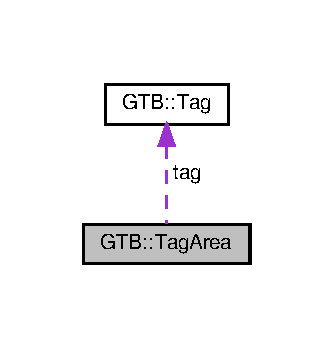
\includegraphics[width=160pt]{a00030}
\end{center}
\end{figure}
\subsection*{Public Member Functions}
\begin{DoxyCompactItemize}
\item 
\mbox{\Hypertarget{a00032_a0454486ec9cbb9734c59471719a3d071}\label{a00032_a0454486ec9cbb9734c59471719a3d071}} 
{\bfseries Tag\+Area} (\hyperlink{a00028}{Tag} tag, Glib\+::\+Ref\+Ptr$<$ Gtk\+::\+Text\+Mark $>$ start)
\item 
\mbox{\Hypertarget{a00032_a60b193884237e460dccde4f45ad4d088}\label{a00032_a60b193884237e460dccde4f45ad4d088}} 
bool {\bfseries operator==} (\hyperlink{a00028}{Tag} tag)
\end{DoxyCompactItemize}
\subsection*{Public Attributes}
\begin{DoxyCompactItemize}
\item 
\mbox{\Hypertarget{a00032_abc21113af3169babd1942ea0dca0977a}\label{a00032_abc21113af3169babd1942ea0dca0977a}} 
\hyperlink{a00028}{Tag} {\bfseries tag}
\item 
\mbox{\Hypertarget{a00032_a1400795c4c72f6e179471216afd17a3f}\label{a00032_a1400795c4c72f6e179471216afd17a3f}} 
Glib\+::\+Ref\+Ptr$<$ Gtk\+::\+Text\+Mark $>$ {\bfseries start}
\end{DoxyCompactItemize}


The documentation for this class was generated from the following file\+:\begin{DoxyCompactItemize}
\item 
\hyperlink{a00005}{gtb.\+h}\end{DoxyCompactItemize}

\hypertarget{a00036}{}\section{G\+TB\+:\+:Window Class Reference}
\label{a00036}\index{G\+T\+B\+::\+Window@{G\+T\+B\+::\+Window}}


Inheritance diagram for G\+TB\+:\+:Window\+:\nopagebreak
\begin{figure}[H]
\begin{center}
\leavevmode
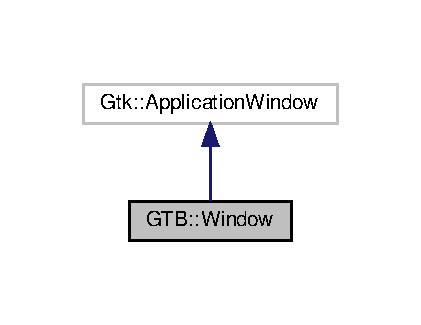
\includegraphics[width=202pt]{a00035}
\end{center}
\end{figure}


Collaboration diagram for G\+TB\+:\+:Window\+:\nopagebreak
\begin{figure}[H]
\begin{center}
\leavevmode
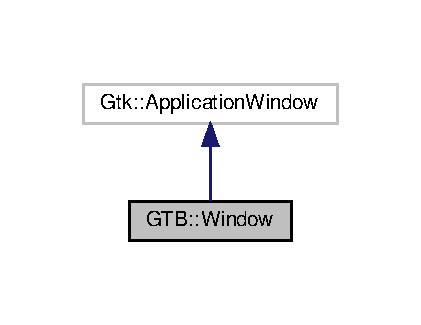
\includegraphics[width=202pt]{a00034}
\end{center}
\end{figure}
\subsection*{Public Attributes}
\begin{DoxyCompactItemize}
\item 
\mbox{\Hypertarget{a00036_a2e64415ee404103528cd33bbdb323fb2}\label{a00036_a2e64415ee404103528cd33bbdb323fb2}} 
Gtk\+::\+Scrolled\+Window {\bfseries scrolled\+\_\+window}
\item 
\mbox{\Hypertarget{a00036_a3fc0002fbdf62b9c1f402b31b8b1568e}\label{a00036_a3fc0002fbdf62b9c1f402b31b8b1568e}} 
Gtk\+::\+Text\+View {\bfseries view}
\item 
\mbox{\Hypertarget{a00036_aed9ad861f7a9c6bdff6df63ea699b1f8}\label{a00036_aed9ad861f7a9c6bdff6df63ea699b1f8}} 
Glib\+::\+Ref\+Ptr$<$ Gtk\+::\+Text\+Buffer $>$ {\bfseries buf}
\item 
\mbox{\Hypertarget{a00036_a0fd9f0ab15e2af9d4963d6e4699f5053}\label{a00036_a0fd9f0ab15e2af9d4963d6e4699f5053}} 
Glib\+::\+Ref\+Ptr$<$ Gtk\+::\+Text\+Mark $>$ {\bfseries outpos}
\item 
\mbox{\Hypertarget{a00036_a942054c00c3266ce86e08b69674bb403}\label{a00036_a942054c00c3266ce86e08b69674bb403}} 
Glib\+::\+Ref\+Ptr$<$ Gtk\+::\+Text\+Mark $>$ {\bfseries instart}
\item 
\mbox{\Hypertarget{a00036_ae5de8dda2b454bbcee99e7dc91ec7a05}\label{a00036_ae5de8dda2b454bbcee99e7dc91ec7a05}} 
Glib\+::\+Ref\+Ptr$<$ Gtk\+::\+Text\+Mark $>$ {\bfseries inend}
\item 
\mbox{\Hypertarget{a00036_a46bb865cf2e4b8efd0f47d37b03b5a77}\label{a00036_a46bb865cf2e4b8efd0f47d37b03b5a77}} 
Glib\+::\+Dispatcher {\bfseries dispatcher}
\item 
\mbox{\Hypertarget{a00036_a52395c2d9848125f2809d0c1b3ed41dc}\label{a00036_a52395c2d9848125f2809d0c1b3ed41dc}} 
std\+::vector$<$ \hyperlink{a00028}{Tag} $>$ {\bfseries table}
\item 
\mbox{\Hypertarget{a00036_ad01f445b4bf1618d14ca83b49c01204e}\label{a00036_ad01f445b4bf1618d14ca83b49c01204e}} 
Glib\+::\+Ref\+Ptr$<$ Gtk\+::\+Text\+Buffer\+::\+Tag\+Table $>$ {\bfseries gtk\+\_\+table}
\end{DoxyCompactItemize}


The documentation for this class was generated from the following file\+:\begin{DoxyCompactItemize}
\item 
\hyperlink{a00005}{gtb.\+h}\end{DoxyCompactItemize}

\chapter{File Documentation}
\hypertarget{a00005}{}\section{gtb.\+h File Reference}
\label{a00005}\index{gtb.\+h@{gtb.\+h}}


Header file for Gnome Text\+Box.  


{\ttfamily \#include $<$signal.\+h$>$}\newline
{\ttfamily \#include $<$errno.\+h$>$}\newline
{\ttfamily \#include $<$unistd.\+h$>$}\newline
{\ttfamily \#include $<$semaphore.\+h$>$}\newline
{\ttfamily \#include $<$fcntl.\+h$>$}\newline
{\ttfamily \#include $<$pthread.\+h$>$}\newline
{\ttfamily \#include $<$sys/stat.\+h$>$}\newline
{\ttfamily \#include $<$gtk/gtk.\+h$>$}\newline
{\ttfamily \#include $<$gdk/gdk.\+h$>$}\newline
{\ttfamily \#include $<$gdk/gdkkeysyms.\+h$>$}\newline
{\ttfamily \#include $<$iostream$>$}\newline
{\ttfamily \#include $<$string$>$}\newline
{\ttfamily \#include $<$exception$>$}\newline
{\ttfamily \#include $<$vector$>$}\newline
{\ttfamily \#include $<$algorithm$>$}\newline
{\ttfamily \#include $<$cstdlib$>$}\newline
{\ttfamily \#include $<$thread$>$}\newline
{\ttfamily \#include $<$chrono$>$}\newline
{\ttfamily \#include $<$glibmm/main.\+h$>$}\newline
{\ttfamily \#include $<$glibmm/iochannel.\+h$>$}\newline
{\ttfamily \#include $<$glibmm/dispatcher.\+h$>$}\newline
{\ttfamily \#include $<$gtkmm/application.\+h$>$}\newline
{\ttfamily \#include $<$gtkmm/applicationwindow.\+h$>$}\newline
{\ttfamily \#include $<$gtkmm/scrolledwindow.\+h$>$}\newline
{\ttfamily \#include $<$gtkmm/textview.\+h$>$}\newline
{\ttfamily \#include $<$gtkmm/textbuffer.\+h$>$}\newline
Include dependency graph for gtb.\+h\+:\nopagebreak
\begin{figure}[H]
\begin{center}
\leavevmode
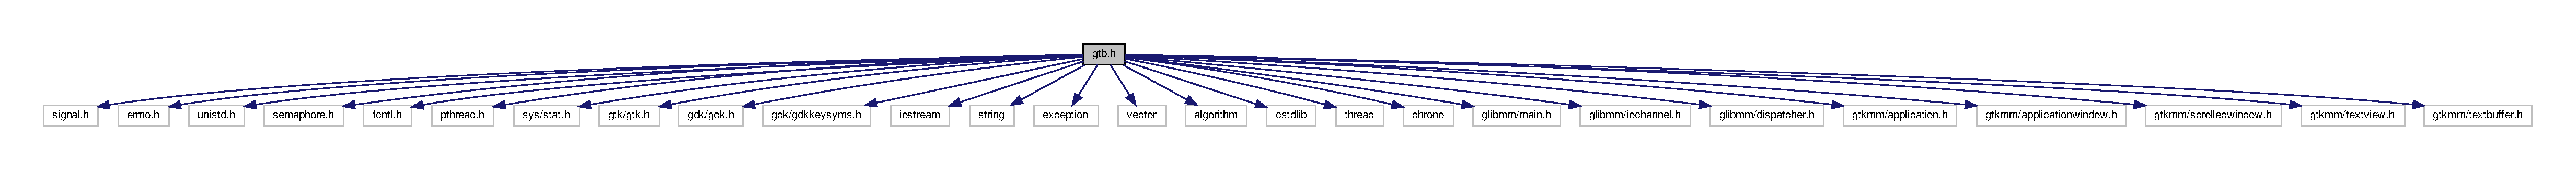
\includegraphics[width=350pt]{a00006}
\end{center}
\end{figure}
\subsection*{Classes}
\begin{DoxyCompactItemize}
\item 
class \hyperlink{a00012}{G\+T\+B\+::\+Error}
\item 
class \hyperlink{a00016}{G\+T\+B\+::\+Fatal\+Error}
\item 
class \hyperlink{a00020}{G\+T\+B\+::\+Sequence}
\item 
class \hyperlink{a00024}{G\+T\+B\+::coord}
\item 
class \hyperlink{a00028}{G\+T\+B\+::\+Tag}
\item 
class \hyperlink{a00032}{G\+T\+B\+::\+Tag\+Area}
\item 
class \hyperlink{a00036}{G\+T\+B\+::\+Window}
\item 
class \hyperlink{a00040}{G\+T\+B\+::\+Outputer}
\item 
class \hyperlink{a00044}{G\+T\+B\+::\+Inputer}
\item 
class \hyperlink{a00048}{G\+T\+B\+::\+Controller}
\end{DoxyCompactItemize}
\subsection*{Macros}
\begin{DoxyCompactItemize}
\item 
\mbox{\Hypertarget{a00005_ac48c337ccf15cdab391eaae729902b5e}\label{a00005_ac48c337ccf15cdab391eaae729902b5e}} 
\#define {\bfseries G\+T\+B\+\_\+\+V\+E\+R\+S\+I\+ON}~1000000L
\item 
\mbox{\Hypertarget{a00005_a6a761932477b582680bf7fed666c6e61}\label{a00005_a6a761932477b582680bf7fed666c6e61}} 
\#define {\bfseries D\+C1}~\textquotesingle{}\textbackslash{}021\textquotesingle{}
\item 
\mbox{\Hypertarget{a00005_a97a74d0dbbdcf880ce8bc1c375c84c32}\label{a00005_a97a74d0dbbdcf880ce8bc1c375c84c32}} 
\#define {\bfseries D\+C2}~\textquotesingle{}\textbackslash{}022\textquotesingle{}
\item 
\mbox{\Hypertarget{a00005_a4877b26a0217c0449768036b0498e78a}\label{a00005_a4877b26a0217c0449768036b0498e78a}} 
\#define {\bfseries D\+C3}~\textquotesingle{}\textbackslash{}023\textquotesingle{}
\item 
\mbox{\Hypertarget{a00005_a3fba98e4f2b44f2762e20abb6578e0d2}\label{a00005_a3fba98e4f2b44f2762e20abb6578e0d2}} 
\#define {\bfseries U\+T\+F8\+\_\+\+C\+H\+A\+R\+\_\+\+M\+AX}~6
\item 
\mbox{\Hypertarget{a00005_a1ac5b819ce482eb4a63e85c3671dd303}\label{a00005_a1ac5b819ce482eb4a63e85c3671dd303}} 
\#define {\bfseries C\+H\+L\+D\+\_\+\+N\+U\+LL}~-\/1
\item 
\mbox{\Hypertarget{a00005_a33309af6aac10118c1d94f9757602a9b}\label{a00005_a33309af6aac10118c1d94f9757602a9b}} 
\#define {\bfseries C\+H\+L\+D\+\_\+\+D\+E\+AD}~-\/2
\item 
\mbox{\Hypertarget{a00005_a7609549a7df0b2ceee442e50a63dc061}\label{a00005_a7609549a7df0b2ceee442e50a63dc061}} 
\#define {\bfseries H1\+\_\+\+S\+C\+A\+L\+E\+\_\+\+S\+I\+ZE}~2.\+0
\item 
\mbox{\Hypertarget{a00005_a6d081c052149a4cb72ba8696174dd6d5}\label{a00005_a6d081c052149a4cb72ba8696174dd6d5}} 
\#define {\bfseries H2\+\_\+\+S\+C\+A\+L\+E\+\_\+\+S\+I\+ZE}~1.\+5
\item 
\mbox{\Hypertarget{a00005_a049f0dd6767e38e4224ca6918ad5b328}\label{a00005_a049f0dd6767e38e4224ca6918ad5b328}} 
\#define {\bfseries H3\+\_\+\+S\+C\+A\+L\+E\+\_\+\+S\+I\+ZE}~1.\+17
\item 
\mbox{\Hypertarget{a00005_aacd6df83c09dfc4d0c289240f32b2f94}\label{a00005_aacd6df83c09dfc4d0c289240f32b2f94}} 
\#define {\bfseries H4\+\_\+\+S\+C\+A\+L\+E\+\_\+\+S\+I\+ZE}~1.\+0
\item 
\mbox{\Hypertarget{a00005_aef63dd05d733d24ce42cdff56955d1fb}\label{a00005_aef63dd05d733d24ce42cdff56955d1fb}} 
\#define {\bfseries H5\+\_\+\+S\+C\+A\+L\+E\+\_\+\+S\+I\+ZE}~0.\+83
\item 
\mbox{\Hypertarget{a00005_ab8d816268208458f38fec00022277704}\label{a00005_ab8d816268208458f38fec00022277704}} 
\#define {\bfseries H6\+\_\+\+S\+C\+A\+L\+E\+\_\+\+S\+I\+ZE}~0.\+67
\end{DoxyCompactItemize}
\subsection*{Functions}
\begin{DoxyCompactItemize}
\item 
\mbox{\Hypertarget{a00005_a2391b249904a79df4d2c8c18807f1f12}\label{a00005_a2391b249904a79df4d2c8c18807f1f12}} 
void {\bfseries G\+T\+B\+::start\+\_\+handler} ()
\item 
\mbox{\Hypertarget{a00005_a21bbd3fc9a78473e3ff815a1173cb3a5}\label{a00005_a21bbd3fc9a78473e3ff815a1173cb3a5}} 
void {\bfseries G\+T\+B\+::exit\+\_\+handler} ()
\item 
\mbox{\Hypertarget{a00005_a4cc5ca0cc64dd02e182a205aa9e43d98}\label{a00005_a4cc5ca0cc64dd02e182a205aa9e43d98}} 
void $\ast$ {\bfseries G\+T\+B\+::handler} (void $\ast$arg)
\end{DoxyCompactItemize}
\subsection*{Variables}
\begin{DoxyCompactItemize}
\item 
\mbox{\Hypertarget{a00005_a5461c31dafd891ad83e4067f7c0f4a2a}\label{a00005_a5461c31dafd891ad83e4067f7c0f4a2a}} 
pid\+\_\+t {\bfseries G\+T\+B\+::pid}
\item 
\mbox{\Hypertarget{a00005_adf9666705cf4df93b7ac84e30e261765}\label{a00005_adf9666705cf4df93b7ac84e30e261765}} 
pid\+\_\+t {\bfseries G\+T\+B\+::cpid}
\item 
\mbox{\Hypertarget{a00005_ad0774f3a41eb220ccdc9a62454107126}\label{a00005_ad0774f3a41eb220ccdc9a62454107126}} 
pthread\+\_\+t {\bfseries G\+T\+B\+::signal\+\_\+handler}
\item 
\mbox{\Hypertarget{a00005_a2547da65375d499a51310ded1bf573ff}\label{a00005_a2547da65375d499a51310ded1bf573ff}} 
Window $\ast$ {\bfseries G\+T\+B\+::windowp}
\item 
\mbox{\Hypertarget{a00005_a4aa97affbe5994c68285edc925c96813}\label{a00005_a4aa97affbe5994c68285edc925c96813}} 
Outputer $\ast$ {\bfseries G\+T\+B\+::outputerp}
\item 
\mbox{\Hypertarget{a00005_acbcc12994db465994d3f1f124aece58f}\label{a00005_acbcc12994db465994d3f1f124aece58f}} 
Inputer $\ast$ {\bfseries G\+T\+B\+::inputerp}
\item 
\mbox{\Hypertarget{a00005_ad22c9e8fc050fba17a9550998ed35a1c}\label{a00005_ad22c9e8fc050fba17a9550998ed35a1c}} 
Controller $\ast$ {\bfseries G\+T\+B\+::controllerp}
\end{DoxyCompactItemize}


\subsection{Detailed Description}
Header file for Gnome Text\+Box. 


%--- End generated contents ---

% Index
\backmatter
\newpage
\phantomsection
\clearemptydoublepage
\addcontentsline{toc}{chapter}{Index}
\printindex

\end{document}
